\head{Сентябрь}{Листок 8. Логика. Теория.}

\textit{Логика} (от древнегреческого logos – слово, выражающее мысль) является началом любой научной теории. В древние века многие философы занимались поисками истины как таковой, изобретая системы аксиом и правила рассуждений. Наиболее известным до нас именем в этой области является Аристотель (384 - 322 гг. до н.э.). Именно Аристотель создал чистую систему силлогизмов– правил вывода, что и привело к возникновению теории логики.\footnote{Математическое исследование этих вопросов берет своё начало от основополагающего труда Джорджа Буля, изданного в Лондоне в 1854 году. Этот труд Буля положил начало математической логики, систематическое развитие
которой было достигнуто работами многих математиков XX века.}
\par
Основная функция логики как науки – изучение того, как из одних утверждений можно выводить другие. Многими правилами логики мы с детства пользуемся неосознанно. Определение, доказательство, опровержение и т.д. – все это функции логики. 
\par
Правила вывода позволяют преобразовывать исходные утверждения подобно тому, как тождественные преобразования в математике дают возможность решать различные системы уравнений. При этом предполагается, что вывод зависит только от способа связи входящих в него утверждений и их строения, а не от их конкретного содержания. Изучая, ''что из чего следует'', логика выявляет наиболее общие или, как говорят, формальные условия правильного мышления. Следующим шагом формализации логики является появление специальной символики для точной и компактной записи утверждений и определения операций над ними. Некоторые такие символы мы уже использовали, с другими символами мы познакомимся позже. 
\par
С появлением языка математической логики стало возможным составлять алгоритмы логического вывода. Стали вести речь о создании искусственного интеллекта. В последнее время логика находит все более широкое применение в технике при исследовании и разработке вычислительных машин, дискретных автоматов. Её методы используются в теории преобразования и передачи информации, теории вероятностей и комбинаторном анализе. Математическая логика находит своё применение в экономике, биологии, медицине, психологии, праве, языкознании.

Решение некоторых логических задач можно описать с помощью таблиц. Вы, скорее всего, уже знакомы с такими методами решения. При решении приходится рассматривать большое количество вариантов, перебирать различные случаи. При этом очень легко что-то потерять, забыть рассмотреть какой-то случай. Чтобы избежать всех этих проблем, математики придумали заносить результаты своих рассуждений в таблицы. Такой метод решения получил название табличной логики. Поясним, в чём заключается этот метод. Допустим, у нас есть три бумажные фигурки: круг, квадрат и треугольник. Они трёх разных цветов: синего, красного и жёлтого. Тогда мы можем нарисовать такую таблицу:

\begin{center}
\begin{tabular}{ | m{3cm} | m{3cm}| m{3cm} | m{3cm} | } 
  \hline
  & красный & синий & жёлтый \\ 
  \hline
  круг &    &   & \\ 
  \hline
  квадрат &    &   & \\ 
  \hline
  треугольник &    &   & \\ 
  \hline
\end{tabular}
\end{center}

Если нам даны ещё какие-то условия про эти фигурки, то мы можем начать расставлять ''плюсы'' и ''минусы'' в эту таблицу. ''Плюс'' означает, что данный вариант реализуется, ''минус'' означает, что не реализуется. Заметьте, что должны быть выполнены следующие условия:

\begin{enumerate}
    \item В каждой строке есть ровно один ''плюс''.
    \item В каждом столбце есть ровно один ''плюс''.
\end{enumerate}

Первое условие означает, что каждый предмет покрашен в один из указанных цветов. Второе – что есть ровно один предмет каждого цвета.

\newpage

\begin{thm}
    Четыре спортсменки – Аня, Валя, Галя и Даша – заняли первые четыре места в соревновании по гимнастике, причём никакие две из них не делили между собой эти места. На вопрос, какое место заняла каждая из спортсменок, трое болельщиков ответили:
    \par
    \textit{Первый:} Аня – второе место. Даша – третье место.
    \par
    \textit{Второй:} Аня – первое место. Валя – второе место.
    \par
    \textit{Третий:} Галя – второе место. Даша – четвёртое место.
    \par
    Оказалось, что каждый из болельщиков ошибся один раз.
    \par
    Какое место заняла каждая из спортсменок?
\end{thm}

\begin{prf}
    Поскольку мы не знаем точно, какое из двух утверждений каждого болельщика верно, а какое ложно, то рассмотрим утверждения первого болельщика и разберём два варианта.
    \par
    \textit{Первый вариант:} ''Аня заняла второе место'' – верно, а ''Даша заняла третье место'' – неверно. 
    \par
    Составим таблицу:
    \begin{center}
    \begin{tabular}{ | m{2cm} | m{2cm}| m{2cm} | m{2cm} | m{2cm} | } 
        \hline
        & 1 & 2 & 3 & 4 \\ 
        \hline
        Аня & -- & + & -- & --\\ 
        \hline
        Валя &  & -- &   &   \\ 
        \hline
        Галя &  & -- &   &   \\ 
        \hline
        Даша &  & -- & -- &   \\ 
        \hline
    \end{tabular}
    \end{center}
    \par
    Запишем ''плюс'' Ане за второе место и отметим ''минусами'' остальные клетки в первой строке и втором столбце. Так как мы договорились, что Аня на втором месте, то утверждение второго болельщика, что Аня заняла первое место, неверно. Но тогда верно его второе утверждение, а именно ''Валя заняла второе место''. Но это невозможно, так как мы решили, что Аня заняла второе место. Значит, этот вариант не подходит, будем разбирать второй.

    \textit{Второй вариант}: ''Аня заняла второе место'' – неверно, а ''Даша заняла третье место'' – верно.
    \par
    Составим таблицу:
    
    \begin{center}
    \begin{tabular}{ | m{2cm} | m{2cm}| m{2cm} | m{2cm} | m{2cm} | } 
        \hline
        & 1 & 2 & 3 & 4 \\ 
        \hline
        Аня &  & -- & -- & \\ 
        \hline
        Валя &  &  & -- &   \\ 
        \hline
        Галя &  &  & -- &   \\ 
        \hline
        Даша & -- & -- & + & -- \\ 
        \hline
    \end{tabular}
    \end{center}

    Запишем ''плюс'' Даше за третье место и отметим ''минусами'' остальные клетки в последней строке и третьем столбце. Так как мы договорились, что Даша на третьем месте, то утверждение третьего болельщика, что Даша заняла четвёртое место, неверно. Но тогда верно его второе утверждение, а именно ''Галя заняла второе место''. Отметим это в таблице:
    
    \begin{center}
    \begin{tabular}{ | m{2cm} | m{2cm}| m{2cm} | m{2cm} | m{2cm} | } 
        \hline
        & 1 & 2 & 3 & 4 \\ 
        \hline
        Аня &  & -- & -- & \\ 
        \hline
        Валя &  & -- & -- &   \\ 
        \hline
        Галя & -- & + & -- & -- \\ 
        \hline
        Даша & -- & -- & + & -- \\ 
        \hline
    \end{tabular}
    \end{center}

    Теперь видно, что ''свободными'' остались только первое и четвёртое места. Значит, это места Ани и Вали. Второй болельщик утверждает, что Валя заняла второе место, но это при наших условиях невозможно. Поэтому это утверждение неверно, но тогда верно, что Аня заняла первое место. Окончательно заполняя таблицу, имеем:

    \begin{center}
    \begin{tabular}{ | m{2cm} | m{2cm}| m{2cm} | m{2cm} | m{2cm} | } 
        \hline
        & 1 & 2 & 3 & 4 \\ 
        \hline
        Аня & + & -- & -- & -- \\ 
        \hline
        Валя & -- & -- & -- & + \\ 
        \hline
        Галя & -- & + & -- & -- \\ 
        \hline
        Даша & -- & -- & + & -- \\ 
        \hline
    \end{tabular}
    \end{center}

    \par

    \textbf{\textit{Решение 2.}} Рассмотрим высказывания второго. Если верно, что Валя заняла второе место, то Аня и Галя не могли занять это место и значит эти утверждения первого и третьего неверны. Но тогда должно быть одновременно верно, что Даша заняли третье место и четвёртое, чего не может быть. Значит, Валя не занимала второго места. Тогда верно, что Аня заняла первое место. Из слов первого следует, что раз утверждение про Аню неверно, то у Даши третье место. Поэтому неверно, что у Даши четвёртое и, следовательно, у Гали второе место, у Вали оставшееся, четвёртое.

    \par

    \textbf{\textit{Ответ:}} Аня – первое место, Валя – четвёртое, Галя – второе и Даша – третье.
\end{prf}

Заметим также, что некоторые логические задачи близки задачам на множества. Действительно, наличие какого-то свойства можно понимать как принадлежность некоторому множеству, а отсутствие – нахождение за пределами рассматриваемого множества.

\begin{figure}[H]
\begin{minipage}{0.64\linewidth}\setlength{\parindent}{1.5em}
    \begin{thm}
        Однажды на лестнице была найдена странная тетрадь. В ней было написано 100 следующих утверждений:
        \par
        «В этой тетради ровно 1 неверное утверждение».
        \par
        «В этой тетради ровно 2 неверных утверждения».
        \par
        «В этой тетради ровно 100 неверных утверждений».
        \par
        Сколько среди этих утверждений верных?
    \end{thm}
\end{minipage}
\hfill
\begin{minipage}{0.25\linewidth}
    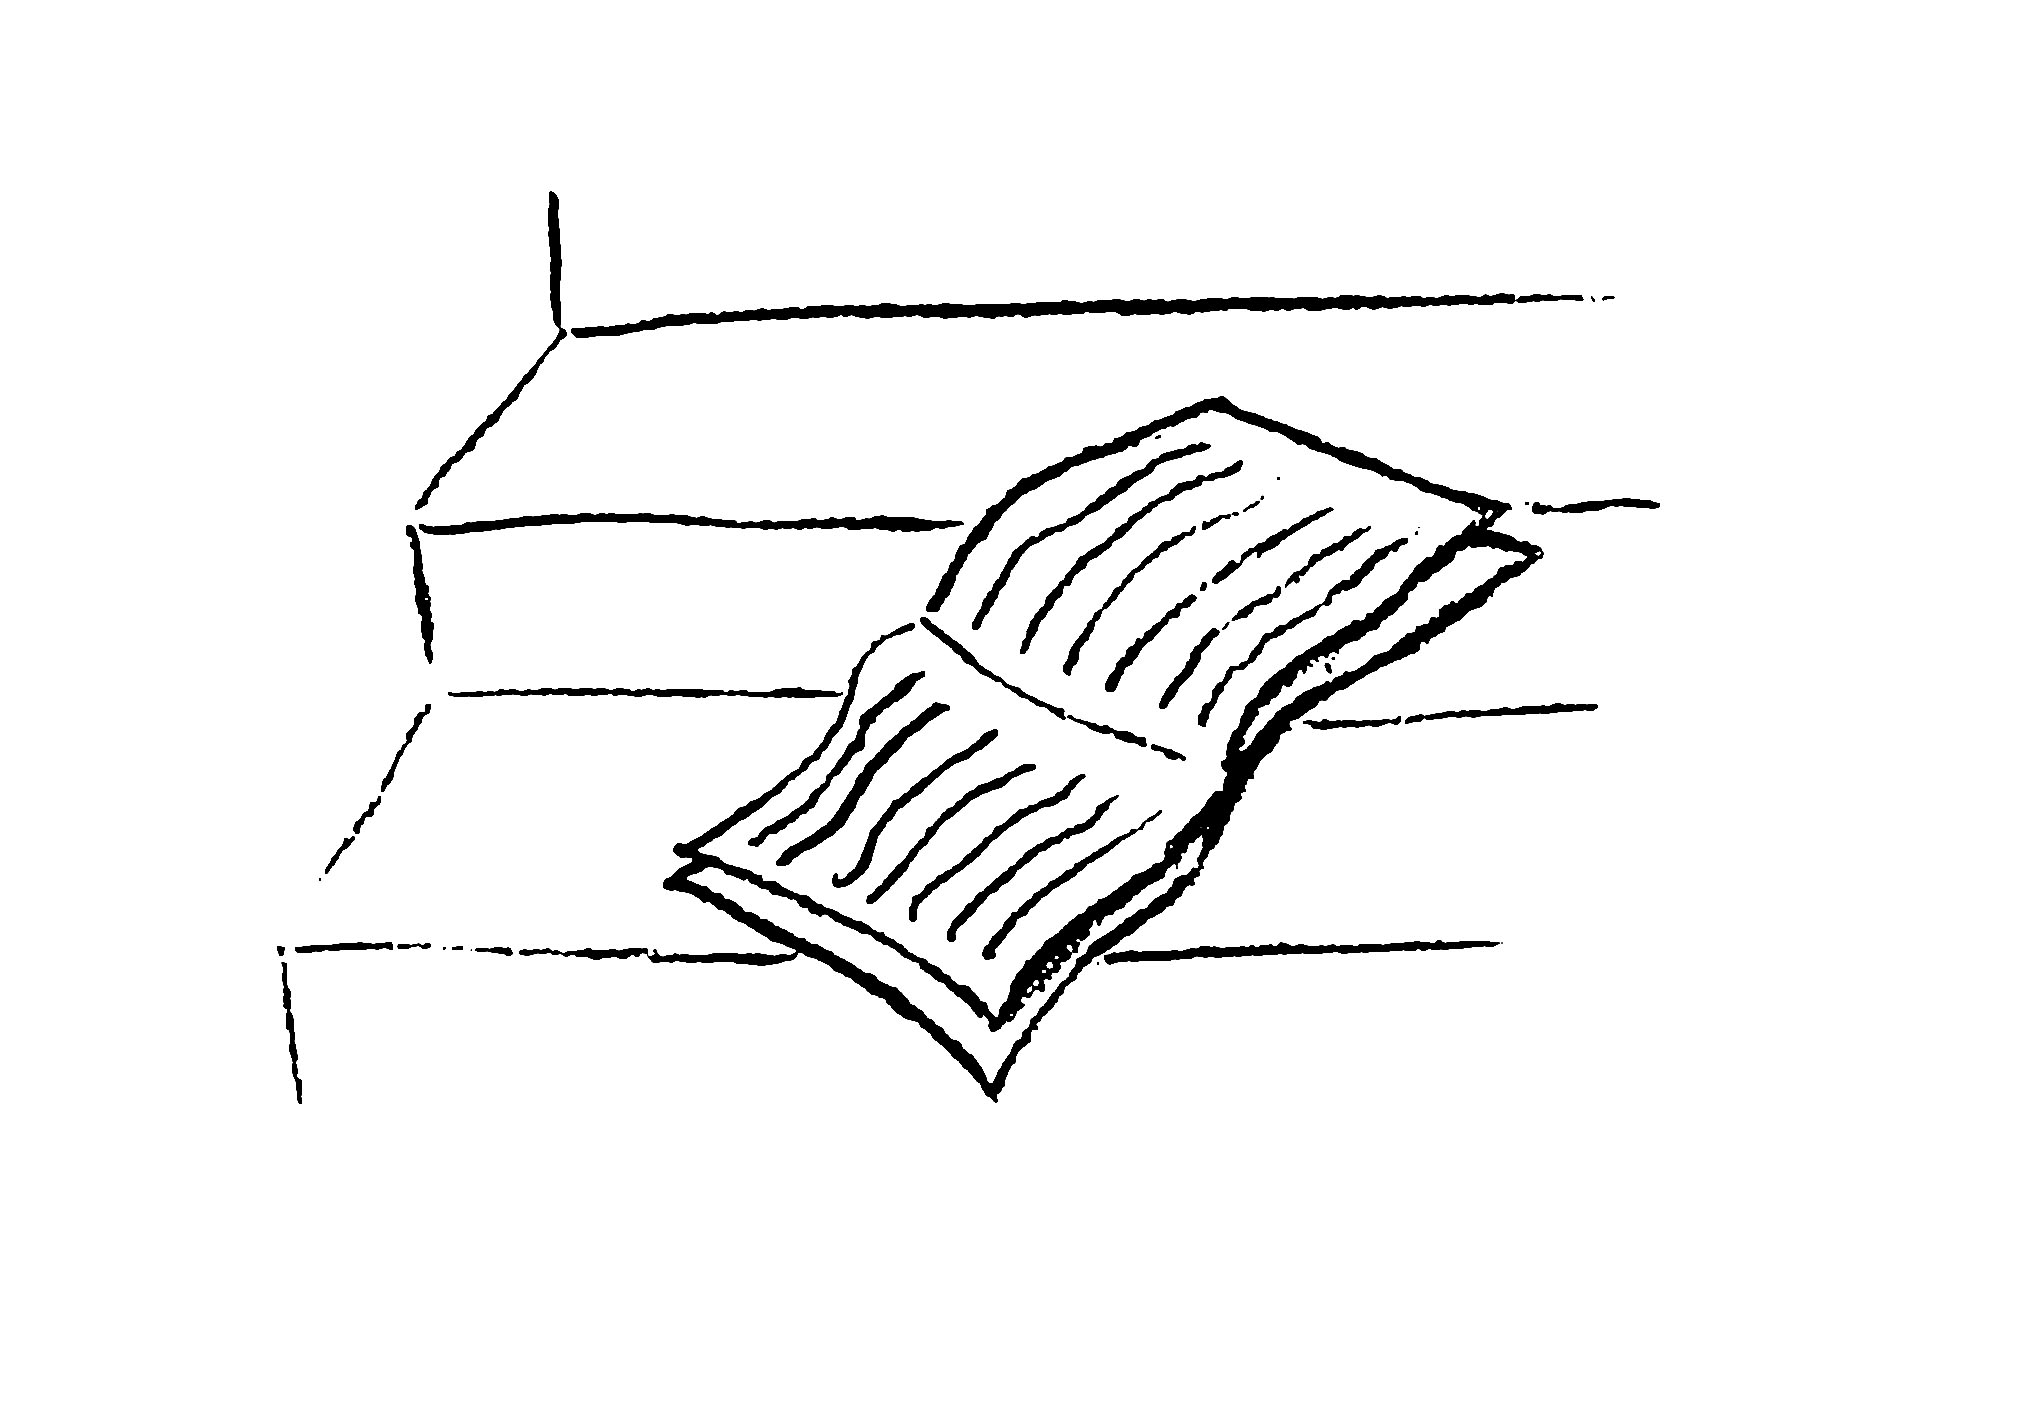
\includegraphics[width=0.95\columnwidth]{img/7.0 1 kniga.jpg}
\end{minipage}
\end{figure} 

\begin{thm}
    В блокноте 10 страниц, на каждой из них написано утверждение: 
    \par
    на первой странице: «В этом блокноте количество неверных утверждений делится на 1»;
    \par
    на второй странице: «В этом блокноте количество неверных утверждений делится на 2»;
    \par
    на третьей: «В этом блокноте количество неверных утверждений делится на 3»;
    \par
    ...
    \par
    на десятой: «В этом блокноте количество неверных утверждений делится на 10».
    \par
    Сколько в блокноте верных утверждений?
\end{thm}

\begin{thm}
    Чего больше: пятниц, кроме тех пятниц, которые не являются тринадцатыми числами, или тринадцатых чисел, кроме тех, которые не являются пятницами?
\end{thm}

\begin{thm}
    Предположим, что справедливы следующие утверждения:
    \par
    а) Среди людей, имеющих обезьянок, есть такие, которые не являются спелеологами.
    \par
    б) Люди, выращивающие кактусы, но не являющиеся спелеологами, не имеют обезьянок.
    \par
    Верно ли тогда, что не все владельцы обезьянок разводят кактусы?
\end{thm}

\begin{thm}
    Известно, что ляпусики, у которых есть варкала, не все бармаглоты. Кроме того, у тех ляпусиков, которые умеют хрюкотать и при этом не бармаглоты, варкал нет. Верно ли, что не все ляпусики, у которых есть варкала, умеют хрюкотать?
\end{thm}

\begin{thm} $^n$
    В тюрьму поместили 2011 узников. Надзиратель сказал им: «Я дам вам вечер поговорить друг с другом, а потом общаться вы не сможете. Иногда я буду одного из вас отводить в комнату, в которой есть лампа (вначале она выключена). Можно её включить или выключить. Если в какой-то момент кто-то из вас скажет мне, что вы все уже побывали в комнате, и будет прав, то я вас освобожу. А если неправ – казню. Если будете молчать, то все побываете в комнате, и ни для кого никакое посещение комнаты не станет последним». 
    \par
    Придумайте стратегию, гарантирующую узникам освобождение.
\end{thm}

\begin{figure}[H]
\begin{minipage}{0.69\linewidth}\setlength{\parindent}{1.5em}
    \begin{thm}
        Эрик увидел двух двухголовых дракончиков, головы которых спутались. Драконы бывают либо правдивые, т.е. все головы говорят только правду, либо лживые, т.е. все головы всегда лгут. Эрик решил помочь дракончикам распутать головы. Но для этого ему надо знать, где чья голова. Он спросил, какая голова чья у дракончиков, на что головы ответили: 
        \par первая голова: «я – правдивая голова»;
        \par вторая голова: «третья голова – моя родная голова»; 
        \par третья голова: «вторая голова – не родная мне голова»; 
        \par четвёртая голова: «третья голова – лживая». 
        \par Какие головы принадлежат каким дракончикам?
    \end{thm}
\end{minipage}
\hfill
\begin{minipage}{0.3\linewidth}
    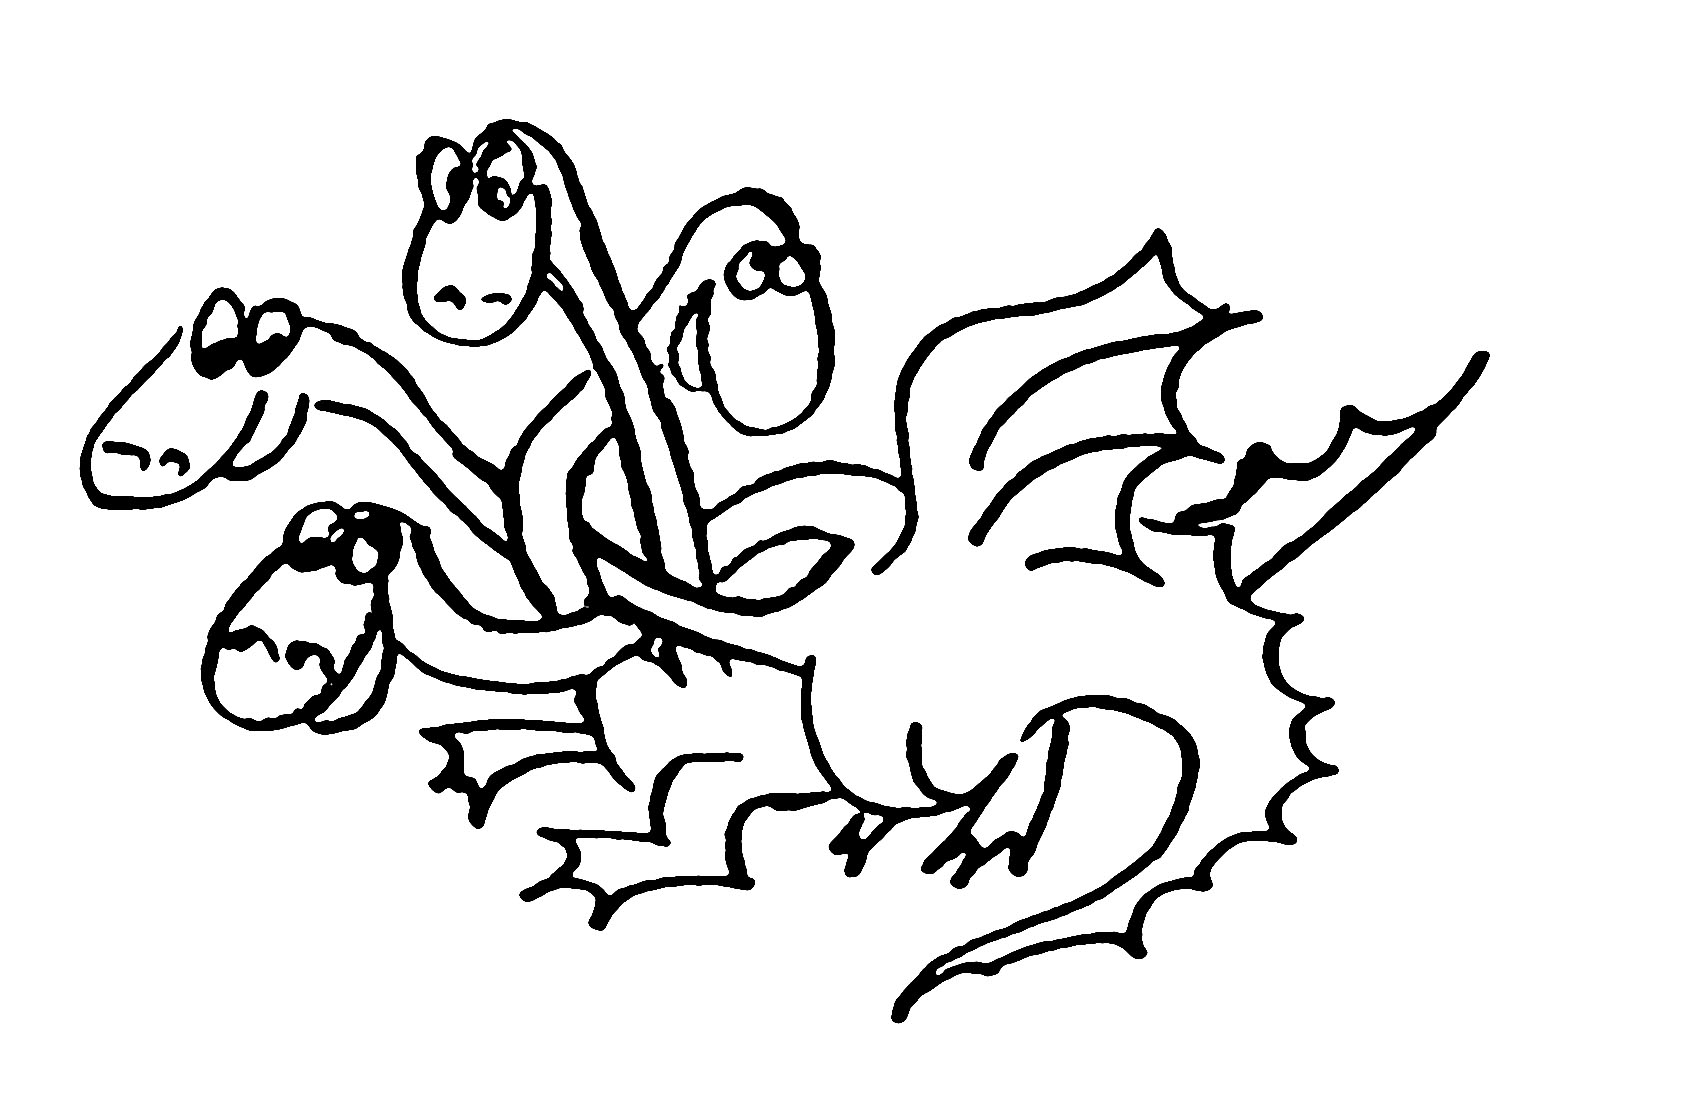
\includegraphics[width=0.95\columnwidth]{img/7.0 2 drakon.jpg}
\end{minipage}
\end{figure} 

\begin{thm} $^*$
    (по мотивам задачи Эйнштейна\footnotemark) В пяти домах с крышами разных цветов на одной стороне улицы живут пять джентльменов, каждый из которых предпочитает определённый напиток, занимается определённым видом спорта и держит животное, птицу, или разводит рыб (напитки, виды спорта и питомцы у всех разные). Известно, что:
    \par \textit{англичанин} живёт в доме с \textit{красной} крышей; 
    \par \textit{швед} держит \textit{собаку};
    \par \textit{датчанин} предпочитает \textit{чай}; 
    \par дом с \textit{зелёной} крышей расположен слева по соседству с домом под \textit{белой} крышей; 
    \par джентльмен из дома под \textit{оранжевой} крышей замечен за игрой в \textit{регби};
    \par \textit{футболист} иногда разговаривает с \textit{попугаем}; 
    \par хозяин дома с \textit{зелёной} крышей пьет \textit{кофе}, а хозяин \textit{среднего} дома – \textit{молоко};
    \par \textit{норвежец} живет в \textit{крайнем} доме, по соседству с домом с \textit{синей} крышей; 
    \par \textit{волейболист} соседствует с \textit{любителем коше}к; 
    \par \textit{любитель лошадей} живет рядом с \textit{регбистом}; 
    \par \textit{немец} играет в \textit{теннис}; 
    \par \textit{сосед волейболиста} пьет только \textit{минеральную воду}, а \textit{баскетболист} предпочитает \textit{квас}.
    \par Выясните, кто в каком доме живёт, каким видом спорта занимается, какие напитки предпочитает, а также кто разводит рыбок.
\end{thm}\footnotetext{Эйнштейн утверждал, что эту задачу не сможет решить более двух процентов мыслящего населения планеты. Интересно, к какой части относитесь вы?}

\section{Высказывания и отрицания.}

\begin{thm}
    Жители города Запузыринска ходят на руках и говорят все наоборот. Например, вместо «здравствуй» они говорят «до свидания», вместо «заходите в гости» – «катись отсюда», а вместо «вышел зайчик погулять» – «зашёл волчище посидеть». А вот какие задачи дают там на уроках математики: «Во вторую ночь заяц выплюнул 100 волков, а в первую – на 5 волков больше. Сколько волков выплюнул заяц в первую ночь?»
    \par
    а) Попробуйте перевести эту задачу на русский язык и дайте ответ.
    \par
    б) Переведите строчку из популярной запузыринской песни: “Огромной берёзе жарко летом”.
\end{thm}

\setlist{nosep} % Убирает вертикальные отступы между айтемами во всех листах


\begin{thm}
    «Все критяне – лжецы», – сказал философ с острова Крит. Какие из следующих утверждений верны, а какие нет, а о каких ничего нельзя сказать? Ответ обоснуйте.
    
    \begin{enumerate}[label=\asbuk*), ref=\asbuk*]
        \item Все критяне – лжецы.
        \item Все критяне говорят правду.
        \item Философ – лжец.
        \item Философ говорит правду.
        \item Среди критян есть лжецы.
        \item Среди критян есть говорящие правду.
    \end{enumerate}
    
\end{thm}


\begin{thm}
    Гоша \textit{верно} решил \textit{все} уравнения. Какие из перечисленных ниже утверждений являются отрицанием этого утверждения?
    
    \begin{enumerate}[label=\asbuk*), ref=\asbuk*]
        \item Петя решил верно все уравнения.
        \item Гоша решил неверно все уравнения.
        \item Гоша решил неверно одно уравнение.
        \item Гоша решил неверно какое-то уравнение.
        \item Гоша решил верно одно уравнение.
        \item Кто-то решил верно все уравнения
        \item Кто-то решил неверно все уравнения.
        \item Кто-то решил неверно какое-то уравнения.
    \end{enumerate}
    
\end{thm}


\begin{thm}
    На Уральском турнире матбоев в \textit{каждом} туре \textit{все} команды решили \textit{все} задачи. Какие из перечисленных ниже утверждений должны быть истинны\footnotemark, чтобы это утверждение стало неверным?
    
    \begin{enumerate}[label=\asbuk*), ref=\asbuk*]
        \item Была команда, которая в каждом туре не решила хотя бы одну задачу
        \item В каждом туре все команды не решили хотя бы одну задачу.
        \item Была команда, которая в каждом туре решила все задачи.
        \item Был тур, в котором ни одна из команд не решила все задачи.
        \item Была команда, которая в одном из туров решила все задачи.
        \item Во всём турнире была задача, которую не решила ни одна команда.
        \item В каждом туре все команды решили хотя бы одну задачу.
    \end{enumerate}
    
\end{thm}\footnotetext{Т.е. истинность этих утверждений является \textit{достаточной}, для того, чтобы сделать вывод.}


\begin{thm}
    На Уральском турнире матбоев \textit{не в каждом} туре \textit{все} команды решили \textit{все} задачи. Пусть это утверждение верно. Какие из перечисленных ниже утверждений обязательно должны быть истинны в этом случае?\footnotemark

    \begin{enumerate}[label=\asbuk*), ref=\asbuk*]
        \item Была команда, которая в каждом туре не решила хотя бы одну задачу
        \item В каждом туре все команды не решили хотя бы одну задачу.
        \item Была команда, которая в каждом туре решила все задачи.
        \item Был тур, в котором ни одна из команд не решила все задачи.
        \item Была команда, которая в одном из туров решила все задачи.
        \item Во всём турнире была задача, которую не решила ни одна команда.
        \item В каждом туре все команды решили хотя бы одну задачу.
    \end{enumerate}
\end{thm}\footnotetext{Т.е. истинность этих утверждений является \textit{необходимой}.}


\begin{thm}
    Назовём контрольную легкой, если за каждой партой найдется ученик, решивший все задачи. Дайте определение \textit{трудной} контрольной.
\end{thm}

\begin{thm}
    Рассмотрим два определения лёгкой контрольной: 
    \par 1) в каждом варианте каждую задачу решил хотя бы один ученик;
    \par 2) в каждом варианте хоты бы один ученик решил все задачи. 
    \par Может ли контрольная быть лёгкой в смысле определения 1) и трудной в смысле определения 2)?
\end{thm}


\section{Логические парадоксы.} 

Мы свободно говорим об истинности утверждений, высказываний... А что такое высказывание?
\par
Например, можно ли что-нибудь сказать об истинности или ложности следующих предложений:

\begin{center}
    \fbox{\begin{varwidth}{0.95\textwidth}
        Утверждение в рамке ложно
    \end{varwidth}}
\end{center}

\begin{center}
    \fbox{\begin{varwidth}{0.95\textwidth}
        \fbox{\begin{varwidth}{0.95\textwidth}
            Утверждение в двойной рамке истинно
        \end{varwidth}}
    \end{varwidth}}
\end{center}

\textit{Высказывание} – это утверждение, о котором можно сказать, истинно ли оно или ложно. Если
какое-то высказывание истинно, то его отрицание\footnote{Если рассматривать утверждения как все возможные события, то само утверждение – это множество некоторых событий, для которых это утверждение справедливо, а отрицание данного утверждения – все события, которые лежат вне этого множества.} ложно (обозначение: $A$ – само высказывание,
$\neg A$ – его отрицание). Понятно, что утверждение ''$A$ или $\neg A$ » всегда истинно (закон исключения третьего, другими словами, третьего не дано), напротив, утверждение ''$A$ и $\neg A$'' всегда ложно (закон противоречия), а двойное отрицание утверждения равносильно самому утверждению: $\neg \neg A = A$ (закон двойного отрицания).

В обычном языке можно придумать много предложений, о которых нельзя сказать, истинны они или ложны. Однако и в рамках логики существуют такие конструкции, о которых нельзя сказать, истинны они или ложны. Такие конструкции называются парадоксами. Например:

\begin{center}
    \begin{tabular}{ | m{6cm} | m{6cm} | } 
        \hline
        \textit{Утверждение справа истинно} & \textit{Утверждение слева ложно.} \\ 
        \hline
    \end{tabular}
\end{center}

\begin{figure}[H]
\begin{minipage}{0.79\linewidth}\setlength{\parindent}{1.5em}
    \begin{thm}
        \textit{(парадокс брадобрея)} Одному солдату отдали приказ брить тех и только тех, кто не бреется сам. Сможет ли он его выполнить?
    \end{thm}
    \begin{thm}
        Существует ли наименьшее целое число, которое нельзя определить при помощи фразы, состоящей не более чем из ста русских слов?
    \end{thm}
    \begin{thm}
        Как-то в 1943 году, шведское радио сообщило о том, что на следующей неделе намечено объявить воздушную учебную тревогу. Чтобы проверить готовность войск ПВО, учение решено провести внезапно так, что даже в день тревоги, ни один человек не сможет предугадать, в котором часу оно будет объявлено. Л. Экбом, преподаватель математики в Стокгольме, усмотрел в этом логический парадокс и обсудил его со своими студентами. Как вам кажется, в чём состоит этот парадокс?
    \end{thm}
\end{minipage}
\hfill
\begin{minipage}{0.2\linewidth}
    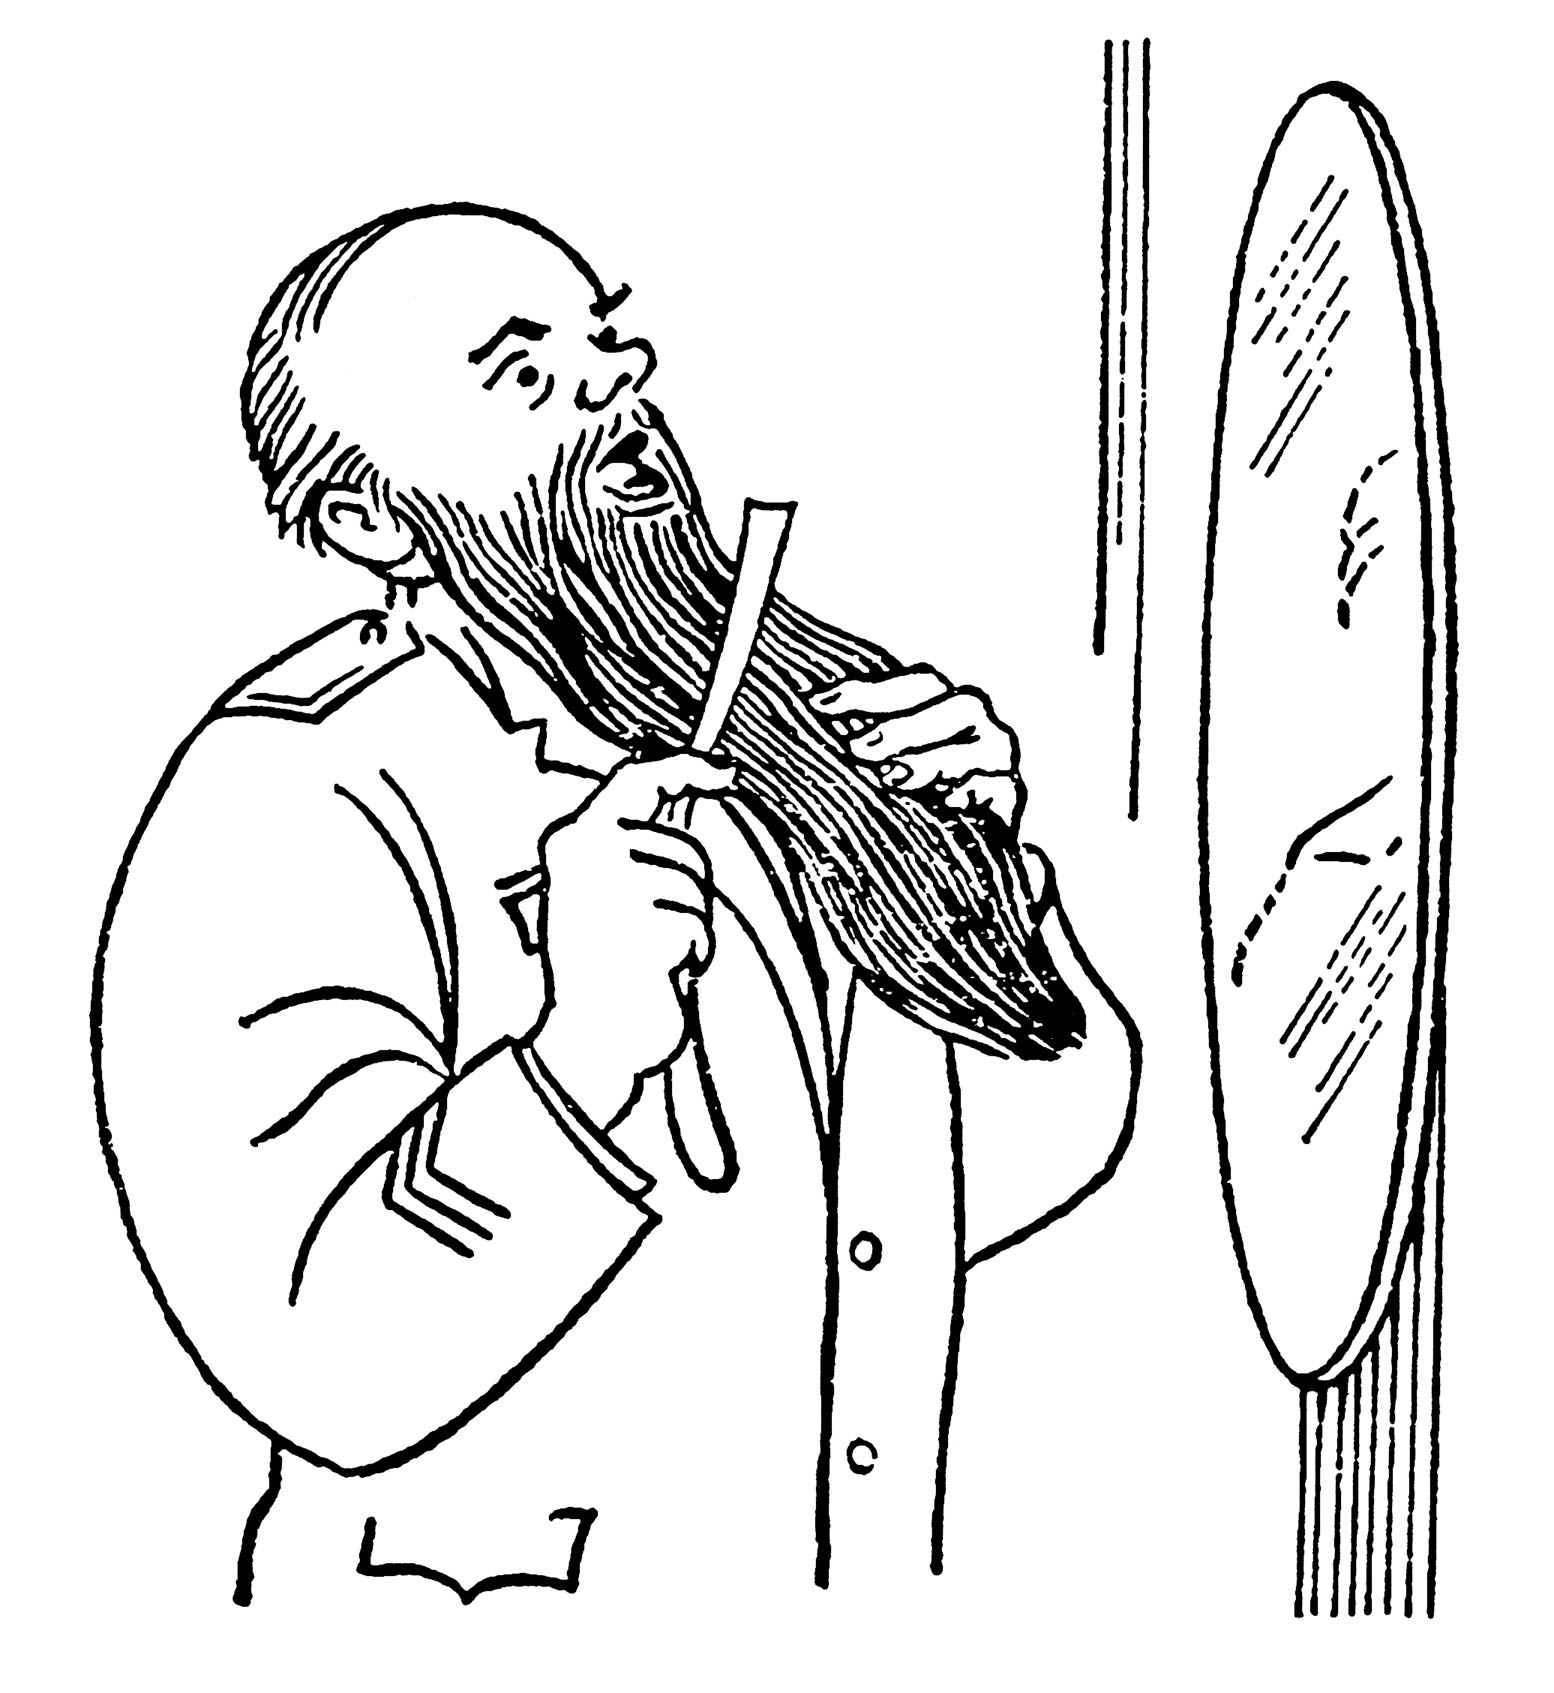
\includegraphics[width=0.95\columnwidth]{img/7.0 3 boroda.jpg}
\end{minipage}
\end{figure} 

\begin{thm}
    Племя людоедов поймало Робинзона Крузо. Вождь сказал: «Мы бы рады отпустить тебя, но по нашему закону ты сначала должен что-нибудь сказать. Если это окажется истиной – мы съедим тебя. Если же это будет ложью – тебя съест наш лев». Как спасти Робинзона?
\end{thm}

\section{Причина и следствие или «Если ... , то ... »}

\epigraph{\textit{«Если дважды два – пять, то существуют ведьмы...»}}{\textit{Феликс Хаусдорф}}

\begin{thm}
    За день до дождя Мюллер всегда чихает. Сегодня Мюллер чихнул. «Завтра будет дождь», – подумал Штирлиц. Прав ли он?
\end{thm}

\begin{figure}[H]
\begin{minipage}{0.79\linewidth}\setlength{\parindent}{1.5em}
    \begin{thm}
    Сформулируйте хотя бы одно
        \begin{enumerate}[label=\asbuk*), ref=\asbuk*]
        \item необходимое и достаточное;
        \item необходимое, но не достаточное;
        \item достаточное, но не необходимое;
        \item не необходимое и не достаточное
        \end{enumerate}
    условие того, что четырехугольник является трапецией.
    \end{thm}
\end{minipage}
\hfill
\begin{minipage}{0.2\linewidth}
    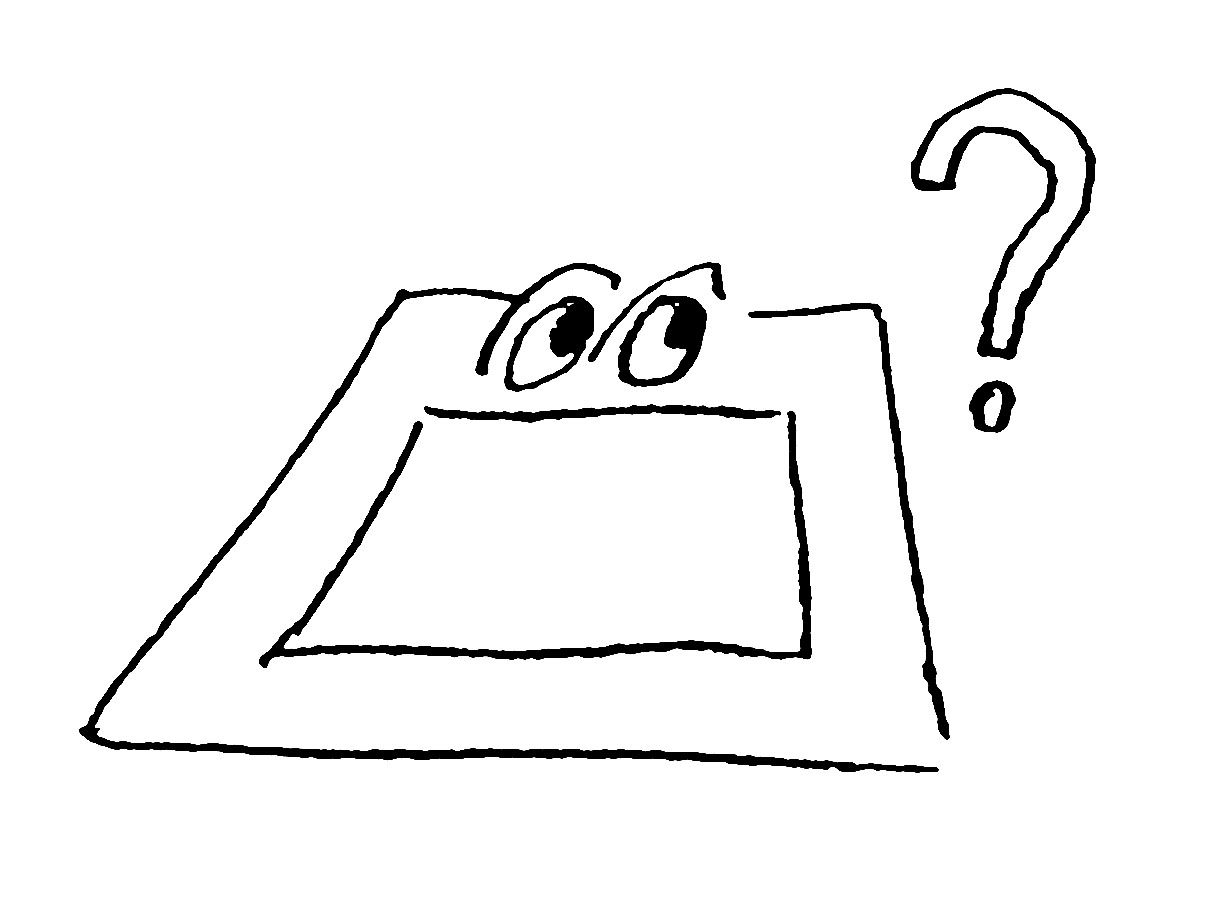
\includegraphics[width=0.95\columnwidth]{img/7.0 4 figura.jpg}
\end{minipage}
\end{figure} 

\begin{thm} \label{8.1 thm1}
    Пусть утверждение $B$: «Этот четырёхугольник – трапеция», а в качестве утверждения $A$ возьмём следующее: «У этого четырёхугольника есть две параллельные стороны». Сформулируйте 8 утверждений:
    \par
    1. Если $A$, то $B$. \hfill 2. Если $A$, то не $B$. \hfill 3. Если не $A$, то $B$. \hfill 4. Если не $A$, то не $B$.
    \par
    5. Если $B$, то $A$. \hfill 6. Если $B$, то не $A$. \hfill 7. Если не $B$, то $A$. \hfill 8. Если не $B$, то не $A$.
    \par
    Какие из этих утверждений верны, а какие нет?
\end{thm}

\begin{thm} \label{8.1 thm3}
    Пусть теперь $A$ и $B$ – какие-то утверждения (каждое из них либо истинно, либо ложно). Рассмотрим восемь теорем:
    \par
    1. Если $A$, то $B$. \hfill 2. Если $\overline{A}$, то $B$. \hfill 3. Если $A$, то $\overline{B}$. \hfill 4. Если $\overline{A}$, то $\overline{B}$.
    \par
    5. Если $B$, то $A$. \hfill 6. Если $\overline{B}$, то $A$. \hfill 7. Если $B$, то $\overline{A}$. \hfill 8. Если $\overline{B}$, то $\overline{A}$.
    \par
    Известно, что теорема 1 верна. Разбейте оставшиеся семь теорем на три группы: те, которые заведомо верны, те, которые заведомо неверны и те, о которых ничего определённо сказать нельзя (т.е. они могут быть верными или неверными в зависимости от выбора утверждений $A$ и $B$).\footnotemark
\end{thm}\footnotetext{Договоримся не рассматривать в качестве $A$ и $B$ утверждения, которые всегда истинны или всегда ложны, например, ''В квадрате все углы тупые'' или ''На плоскости прямые параллельны или пересекаются''.}

Заметим, что предыдущую задачу можно интерпретировать на языке множеств. Т.к. в высказывании речь идёт о некоторых объектах, то по отношению, скажем, к высказыванию $A$ все эти объекты можно разбить на два множества: множество объектов, для которых высказывание верно и множество, для которых неверно. Так сказать, $A$ и $\overline{A}$. (Например, утверждение $A$: «Данный четырёхугольник – параллелограмм», утверждение $B$: «данный четырёхугольник имеет равные стороны».) Тогда что на языке множеств означает наша теорема 1? Только то, что если объект принадлежит множеству $A$, то он принадлежит и множеству $B$!

\begin{thm} $^*$
    Какой смысл по-вашему мнению имеет высказывание Феликса Хаусдорфа, вынесенное в эпиграф?
\end{thm}

\begin{thm} \label{8.1 thm2}
    Однажды утром метеостанция маленького города Новозыбкова передала необычный прогноз погоды. Этот прогноз состоял из нескольких утверждений:
    \begin{enumerate}
        \item Если сегодня дождя не будет, то завтра будет ветреная погода.
        \item Если сегодня пойдёт дождь, то завтра без осадков.
        \item Если сегодня будет холодно, то влажность воздуха сегодня будет высокой.
        \item Если сегодня будет тепло, то завтра безветренно.
        \item Если сегодня ветра нет, то завтра будет тепло при высокой влажности и дождь.
        \item Если сегодня ветреная погода, то завтра – низкая влажность воздуха, но будет дождь.
        \item Если сегодня влажность будет высокой, то завтра она останется без изменений.  
    \end{enumerate}
    Допустим, что каждое утверждение синоптиков верно. Определите в этом случае погоду (т.е. температуру, осадки, влажность и ветер) на сегодня и завтра.
\end{thm}


\begin{center}
    \textit{\textbf{Лирическое отступление.}}
\end{center}

В курсе геометрии вы доказывали следующие утверждения: «Если четырёхугольник – параллелограмм, то его стороны попарно равны.», «Если четырёхугольник – параллелограмм, то его диагонали делятся точкой пересечения пополам.» Отсюда справедливо утверждение: «Если четырёхугольник – параллелограмм, то его стороны попарно равны и диагонали делятся точкой пересечения пополам».
Рассмотрим ещё один пример. В школьной столовой сок стоит 3 руб., а булочка – 2 руб. Справедливы следующие утверждения: «Если у Полины есть 3 рубля, то она может купить булочку.», «Если у Полины
есть 3 рубля, то она может купить сок.» Отсюда справедливо утверждение: «Если у Полины есть 3 рубля, то
она может купить булочку и сок.» ... Рассуждения аналогичны. В чём тут дело?

\section{«Сложносочинённые» утверждения.}

Пусть имеется набор некоторых высказываний, про которые можно узнать, истинны они или ложны. Будем обозначать их заглавными буквами: $A$, $B$, $C$ и т.д. Как и в обычном языке, из уже имеющихся высказываний можно, как из кирпичиков, строить новые. Например, в задачах \ref{8.1 thm1} – \ref{8.1 thm2} высказывания были построены с помощью конструкции «если $A$, то $B$»\footnote{В этом случае высказывание $A$ называется посылкой, а высказывание $B$ – следствием или заключением}. Как из простых предложений можно строить сложносочинённые предложения, где все входящие предложения равноправны, так и из «простых» высказываний можно строить сложные с помощью союзов «и» и «или».

\begin{dfn}
    Пусть $A$ и $B$ – некоторые высказывания. Тогда $A \vee B$ – \textit{дизъюнкция (логическое сложение)} высказываний $A$ и $B$. (Читается «$A$ или $B$» ) Это высказывание истинно, когда хотя бы одно из входящих в него простых высказываний истинно, а ложно, когда ложны все высказывания.
\end{dfn}

\begin{dfn}
    Аналогично, $А \& \ В$\footnote{Также используется обозначение $A \wedge B$.} – \textit{конъюнкция (логическое умножение)} высказываний $A$ и $B$. (Читается «$A$ и $B$» ) Это высказывание истинно только когда истинны все входящие в него высказывания, а ложно, когда ложно хотя бы одно.
\end{dfn}

Для наглядности запишем в табличку:

\begin{figure}[H]
\begin{minipage}{0.45\linewidth}\setlength{\parindent}{1.5em}
    \begin{center}
        \begin{tabular}{ |c|c|c| } 
            \hline
             $A$ & $B$ & $A \vee B$ \\ 
             \hline
             \textit{истина} & \textit{истина} & \textit{истина} \\ 
             \hline
             \textit{истина} & \textit{ложь} & \textit{истина} \\ 
             \hline 
             \textit{ложь} & \textit{истина} & \textit{истина} \\ 
             \hline 
             \textit{ложь} & \textit{ложь} & \textit{ложь} \\ 
             \hline
        \end{tabular}
    \end{center}
\end{minipage}
\hfill
\begin{minipage}{0.45\linewidth}
    \begin{center}
        \begin{tabular}{ |c|c|c| } 
            \hline
             $A$ & $B$ & $A\  \& \ B$ \\ 
             \hline
             \textit{истина} & \textit{истина} & \textit{истина} \\ 
             \hline
             \textit{истина} & \textit{ложь} & \textit{ложь} \\ 
             \hline 
             \textit{ложь} & \textit{истина} & \textit{ложь} \\ 
             \hline 
             \textit{ложь} & \textit{ложь} & \textit{ложь} \\ 
             \hline
        \end{tabular}
    \end{center}
\end{minipage}
\end{figure} 

Почему эти операции называют сложением и умножением станет понятнее, если считать значение «истина» равным 1, а значение «ложь» – 0.\footnote{Правда, при сложении нам придется договориться, что 1 + 1 = 1.}

\begin{ex}
    Решите примеры:
    \par
    \textbf{1}. 1 $\vee$ 0 = ? \hfill 
    \textbf{2}. 0 $\&$ 1 = ? \hfill
    \textbf{3}. 1 $\&$ (0 $\vee$ 1) = ? \hfill
    \textbf{4}. (1 $\&$ 1) $\vee$ (0 $\vee$ 1) = ? \hfill
    \textbf{5}. 0 $\vee$ (0 $\vee$ (0 $\vee$ 1)) = ?
\end{ex}

\begin{ex}
    Вычислите значение выражения, если $A$ истинно, а $B$ - ложно:
    \par
    \textbf{1}. $B$ $\vee$ $A$ \hfill 
    \textbf{2}. $A$ $\&$ $\overline{B}$ \hfill
    \textbf{3}. $A$ $\&$ ($\overline{A}$ $\vee$ $\overline{B}$) = ? \hfill
    \textbf{4}. ($\overline{A}$ $\&$ $\overline{B}$) $\vee$ ($\overline{A}$ $\vee$ $B$) \hfill
    \textbf{5}. $\overline{A}$ $\vee$ ($\overline{B}$ $\vee$ ($B$ $\vee$ $A$))
\end{ex}

\begin{thm}
    Антон лжёт по понедельникам, вторникам и средам, а в остальные дни говорит только правду. Выясните, в какие дни недели Антон может заявить:
    \par а) Я лгал вчера и буду лгать завтра.
    \par б) Я лгал вчера или буду лгать завтра. 
    \par в) Я не лгал вчера и не буду лгать завтра.
    \par г) Я не лгал вчера или не буду лгать завтра.
\end{thm}

\begin{thm}
    Известно, что утверждение «$A$ или не $B$» истинно. Что вы можете сказать про истинность утверждений $A$ и $B$. А если утверждение «$A$ или не $B$» ложно?
\end{thm}

\begin{thm}
    На улице \textit{светит солнце} и у Оли \textit{плохое} настроение. Какие из перечисленных ниже утверждений являются отрицанием этого утверждения?
    \begin{enumerate}[label=\asbuk*), ref=\asbuk*]
        \item На улице пасмурно и у Оли хорошее настроение.
        \item На улице пасмурно или у Оли хорошее настроение.
        \item На улице пасмурно и у Оли плохое настроение.
        \item На улице пасмурно или у Оли плохое настроение.
        \item На улице светит солнце и у Оли хорошее настроение.
        \item На улице светит солнце или у Оли хорошее настроение.
    \end{enumerate}
\end{thm}

\begin{thm}
    На уроке алгебры Андрей получил \textit{пятёрку или четвёрку}. Какие из перечисленных ниже утверждений являются отрицанием этого утверждения?
    \begin{enumerate}[label=\asbuk*), ref=\asbuk*]
        \item На уроке алгебры Андрей получил пятёрку и четвёрку.
        \item На уроке алгебры Андрей получил двойку и тройку.
        \item На уроке алгебры Андрей получил двойку или тройку.
        \item На уроке алгебры Андрей не получил пятёрку и не получил четвёрку.
        \item На уроке алгебры Андрей не получил пятёрку или не получил четвёрку.
        \item На уроке алгебры Андрей получил пятёрку, но не получил четвёрку.
        \item На уроке алгебры Андрей не получил пятёрку, но получил четвёрку.
    \end{enumerate}
\end{thm}

\begin{dfn}
    Пусть $А$ и $В$ – некоторые высказывания. Конструкция «если ... , то ... » называется \textit{логическим следованием} или \textit{импликацией}. Обозначение $А \Rightarrow В$.
\end{dfn}

\begin{ex}
    Составьте табличку значений для импликации и сравните полученные результаты с результатом задачи \ref{8.1 thm3}.
\end{ex}